\documentclass[conference]{IEEEtran}

\usepackage{etoolbox}
\usepackage{graphicx}
\usepackage[numbers]{natbib}
\bibliographystyle{IEEEtranN}
\usepackage{url}
\usepackage{float}
\usepackage[listings,skins]{tcolorbox}
\usepackage{amsmath}

\begin{document}
\title{Risk in \\Open-Source Projects\\
{\footnotesize Technical Document - INSERT DATE FINISHED}
}

\author{\IEEEauthorblockN{Róisín Ní Bhriain}
\IEEEauthorblockA{Student Number: 23269640}
\and
\IEEEauthorblockN{Sneha Dechamma Mallengada Suresh}
    \IEEEauthorblockA{Student Number: 23262168}}

\maketitle
\thispagestyle{plain}
\pagestyle{plain}

\begin{abstract}
Measuring risk is essential in ensuring the security, reliability and compliance of software systems. Open-source software is both transparent and accessible but may nevertheless be vulnerable to security risks such as software vulnerabilities. Open-source software thus requires analysis to identify and mitigate these risks prior to adoption. Developers and organisations need to understand the risks associated with their open-source supply chain to safeguard against any data breaches or other attacks. Making informed decisions on software adoption by analysing the risks in their open-source dependencies is an important part of this. This paper explores, proposes and evaluates methods for assessing risk prior to adopting open-source software. There are a number of objects of analysis used to rate risk such as measuring project activity and vulnerability data and our aim is to combine them to give a more comprehensive view of the risks of using a particular open-source project. We examine the literature to decide on an appropriate algorithm for each measure of risk. We develop a tool to forecast the risks in dependency trees using ARIMA prediction by analysing project activity and vulnerabilities. A dependency graph is generated to aid in identifying where the risk lies in Maven dependency trees. 
\end{abstract}

\begin{IEEEkeywords}
ARIMA prediction, software vulnerabilities, Maven dependency trees.
\end{IEEEkeywords}

\section{Introduction}
In 2005 it was found that 87\% of US companies and government agencies rely on open-source software \cite{i_ceh_analysis_2021}. The popularity of open-source software in large software projects has increased in the last number of years \cite{zajdel_open_2022} and over 3.6 million repositories depend on the top 50 open-source projects \cite{subramanian_empirical_2020}. Open-source software has many benefits. The reuse of libraries can reduce development efforts substantially for developers as they do not have to spend time working on problems already solved. The use of open-source libraries is unrestricted and transparent which means developers can modify and distribute the code according to their needs. The reuse of libraries - open-source or otherwise - can create a list of dependencies called a supply chain. The supply chain is a chain of dependencies, which can include open-source software. The supply chain involves a network of participants who perform activities on the dependencies \cite{k_singi_trusted_2019}. As software projects grow larger so do the supply chains and thus they can become difficult to manage leading developers to turn to package managers like Maven for Java projects. In Java in particular, the average application depends on about 40 third-party libraries \cite{a_m_mir_effect_2023}, in comparison to C/C++ repositories which rely on 6.3 third-party libraries on average \cite{tang_towards_2023}.

With the increased use of open-source software, attackers have begun to exploit known vulnerabilities in trusted components in the supply chains by injecting malicious code into software packages \cite{ohm_backstabbers_2020}. The number of these types of attacks has been increasing with 34\% of all recorded supply chain attacks taking place in 2020 and 66\% of all recorded supply chain attacks occurring in 2021 \cite{m_z_malik_protection_2023}. These attacks can come at a great cost to users of open-source software with data breaches in particular coming at a cost of \$388 million on average for a breach of 50 million data records \cite{x_wang_feasibility_2021}. Once vulnerabilities are discovered, it is important that users of open-source software identify whether they are impacted by the reported vulnerabilities or by inactivity in the open-source projects. 

Prediction of risk is a technique that can be used to measure whether certain open-source projects are worth using when measuring the quality of the software \cite{abunadi_towards_2015}. Several objects of analysis are used to predict this type of risk. Some of the key techniques in the prediction of risk in open-source software include the prediction of vulnerabilities using code metrics, the prediction of project activity on version control systems such as GitHub, and the prediction of the number of vulnerabilities released on vulnerability databases such as the National Vulnerability Database (NVD). For the purpose of this paper, we focused on the prediction of project activity and the number of vulnerabilities per month as these have been found to be promising \cite{xia_predicting_2022, s_wu_vulnerability_2020}. 

At present, most of the existing research focuses on one specific object of analysis such as project activity or vulnerability data. This paper explores the prediction of risks in Maven dependency trees by examining both GitHub project activity and NVD Common Vulnerabilities and Exposures (CVE) data. We aim to use Time Series forecasting, or more specifically, we aim to use ARIMA prediction for both sets of data based on user configuration data that returns a coloured graph based on the analysed risk. The creation of a tool like this could help users identify any vulnerable components in their supply chain so they can find an alternative component which is not as risky \cite{noauthor_open_nodate}. 

The structure of this paper is as follows: we first explore the literature on the prediction of risk in open-source software focusing in particular on both project activity predictions and vulnerability predictions. We then explore some case studies where a tool to explore risk in dependency trees would have been useful for users to identify risky modules. We describe the data from APIs that we used as well as the different predictions we made. Finally, we describe the calculations and algorithms we used when predicting risk according to user-assigned metrics and the results that we obtained. 
\\\\
We will answer the following research questions:\\

\begin{itemize}
    \item \textit{RQ1:} Can we provide developers with an effective risk measure when choosing between multiple candidate open-source components?\\
    \item \textit{RQ2:} Can a visual dependency tree be created for a project consisting of colour-coded nodes based on the predicted risks?\\
\end{itemize}

By answering the above questions we aim to provide some new insights on the area of risk prediction for Maven projects. 

\section{Related Work}
In this section, we review relevant work in the prediction of risk in open-source software. We examine the machine learning models used as well as the different objects of analysis used in the predictions.  

\subsection{Vulnerability Propagation}
Roughly 1.2\% of projects directly use vulnerable code in their dependencies \cite{a_m_mir_effect_2023}. However, a small number of vulnerable packages such as \textit{jackson-databind} and \textit{netty-codec-http} could affect up to 375,607 packages in the Maven ecosystem. This means CVEs can affect a large number of Maven projects. In \cite{c_liu_demystifying_2022} the authors present a dependency vulnerability graph of the entire NPM ecosystem. In investigating the JavaScript NPM ecosystem the authors propose an algorithm to resolve dependency trees as well as vulnerability propagation paths. They find that vulnerabilities affect up to 16.7\% of third-party libraries in their current versions. Some widely known CVEs exist in the current dependency trees of a significant number of packages. As packages grow larger and more dependencies are added the complexity of discovering vulnerable dependencies increases. The complexity can be reduced from an exponential to polynomial level depending on the number of relationships through a search algorithm based on lazy strategy \cite{w_hu_open_2019}. The authors also propose the use of optimal blocking analysis to complete vulnerability repair for a project with minimal blocking. Blocking analysis finds the cost of repairing an entire propagation path where each dependencies depend on an affected module - each dependency must be updated after a repair is made. 

\subsection{Project Metadata Analysis}
One of the main indicators of an open-source project's survival is project activity. In addition to project activity level, community size and time-to-fix bugs, subscriber base was identified as a measure of the success of an open-source project \cite{sen_open_2012}. Measuring project activity in open-source software provides a means of predicting the success and security of projects. In \cite{l_bao_large_2021} the authors examine the contributors in open-source projects and use several machine learning and deep learning techniques to predict their activity. They attempt to differentiate between newcomers who leave a project after a short time and those who stay for a long time. Some of the most important features are the number of project followers, the programming language and the average number of commits per developer. A dataset from GitHub as well as a survey conducted among developers were used to identify factors affecting long-term contributors. Predicting the health of an open-source project is explored in \cite{xia_predicting_2022}. Data from over one thousand GitHub projects was used to predict multiple health indicators using machine learning and the error rate was reduced using hyperparameter optimisation. Predictions included the number of contributors, the number of commits, and the number of pull requests and issues. These metrics are indicative of the project’s overall activity level. The authors also conducted a survey which indicated that the number of contributors, commits, and pull requests are real-world concerns for developers. The commit activity of individuals can also be forecasted as active developers play a significant role in the survival of open-source projects. Fewer than 50\% of abandoned projects find new contributors and so contributor retention is a major indicator of a project's health. A simple probabilistic model can be used to predict the time until the next contribution for specific contributors in a project \cite{decan_gap_2020}. Committing is an important activity in open-source projects and the standard measurement is \textit{number of commits per month}. ARIMA is the most popular prediction method in predicting commits per month \cite{chahal_fuzzy_2016}.

\subsection{Vulnerability CVE Data Analysis}
Time series forecasting is a popular method for predicting vulnerabilities. In \cite{gencer_time_2021} the authors analyse the use of an autoregressive integrated moving average (ARIMA) model to predict vulnerabilities. Data on vulnerabilities from the NVD was analysed \cite{noauthor_vulnerability_nodate}. The National Vulnerability Database (NVD) is a database maintained by the National Institute for Technology which maintains details on known vulnerabilities. The authors aimed to predict the number of Android vulnerabilities per month. The authors compared ARIMA's performance with the long short-term memory model (LSTM), artificial neural network (ANN) and recurrent neural network deep learning techniques and found ARIMA gives better results. They found the LSTM to have comparable error rates with ARIMA and to have more successful results than the two deep learning techniques. Another paper discusses the use of ARIMA to predict vulnerabilities \cite{pokhrel_cybersecurity_2017}. They use a linear and a non-linear approach comparing ARIMA and Artificial Neural Networks and Support Vector Machines (SVM) again using reported vulnerabilities from the NVD for three different operating systems. The results indicated that there were sharp fluctuations in the number of vulnerabilities, the non-linear approaches were a better predictor, however, the ANN did not have sufficient data to perform well. The authors of \cite{roumani_time_2015} used two methods of time series analysis to predict vulnerabilities for web browsers: ARIMA and exponential smoothing. The trend, level and seasonality of the vulnerabilities were considered to help in prediction. They note that level was the only significant parameter. Datasets from the NVD were also used in this study. The prediction of the number of CVEs published in the NVD per month can be done using a number of different machine-learning models but it must be noted that the best predictor may change over time as the data changes. In \cite{leverett_vulnerability_2021} they explore 11 different models to forecast the number of CVEs and they note that most models fall flat at the three month mark. These predictions are done on the NVD and predict the vulnerabilities for every project per month rather than focusing on just one project or dependency. 

\subsection{Research Gap}
A research gap stems from the fact the papers above each focus on a single specific object of analysis (project activity or NVD) and thus do not produce a measurement of the overall health of a dependency. A dependency with many vulnerabilities and significant project activity may be deemed less risky by users than a dependency with low project activity and few vulnerabilities. The use of vulnerability prediction models to predict across multiple projects is also a gap in the research and it could certainly be useful when predicting risk in dependency trees. 

\section{Case Studies}
In this section, we will identify a number of case studies where a tool like ours would have been valuable in rapidly identifying high-risk dependencies in a project. 

\subsection{Log4j}
In November 2021 a vulnerability was discovered in the popular open-source logging library Apache Log4j. This software is widely used in Java projects and web portals. The vulnerability in this package meant that hackers could run malicious code remotely on a victim's machine \cite{h_gupta_identification_2022}. The main aim of the log4j exploit is to obtain Lightweight Directory Access Protocol information and this will serve as a gateway to full control of the machine. The attack consists of several steps: information gathering, weaponisation, delivery, exploitation and installation \cite{f_maulana_unmasking_2023}. Numerous projects were unaware that they were affected by the Log4j vulnerability as their dependencies included the Log4j library and a graph of risk dependency risks such as that generated by our software would have helped them discover that they were vulnerable. Once the Log4j vulnerability was reported a user could have used our algorithm to verify that some of their dependencies have vulnerabilities and taken steps to find an alternative library. 

\subsection{Heartbleed Vulnerability}
In April 2014 the Heartbleed vulnerability was discovered in OpenSSL versions 1.0.1 and 1.0.1f. OpenSSL is a popular open-source cryptography library. The vulnerability relates to the established connection being kept "alive" through \textit{Heartbeat} messages. Hackers could craft a similar message to the official \textit{Heartbeat} Message and exploit a buffer overflow to obtain private information in response \cite{s_kyatam_heartbleed_2017}. It was estimated that 24-55\% of HTTPS servers in the Alexa Top 1 million were vulnerable and even 48 hours after the disclosure of the vulnerability around 11\% remained vulnerable as they did not take action to mitigate the attack. This attack could reveal sensitive data such as private keys and only 10\% of affected servers changed their TLS certificates and of these 14\% did not replace their private keys thus gaining no protection \cite{durumeric_matter_2014}. A number of affected servers were unaware they were affected so a tool such as the one we propose would have been useful in ascertaining whether they were vulnerable to Heartbleed. 

\begin{figure}
\begin{center}
    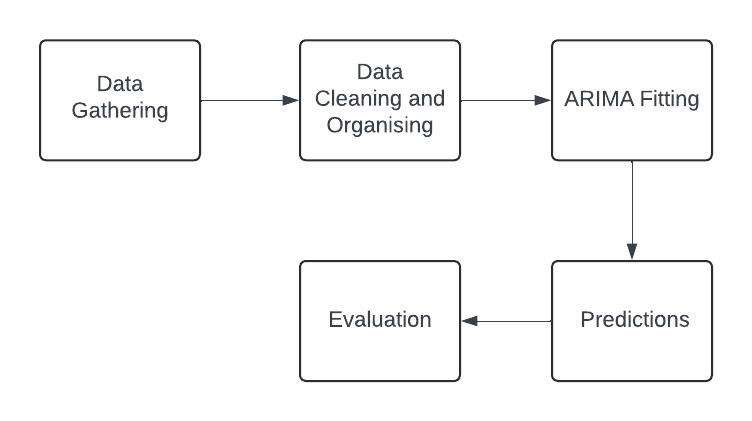
\includegraphics[scale=0.5]{Pipeline.png}
    \caption{The Time Series Pipeline.}
    \label{fig:pipeline}
\end{center}
\end{figure}

\section{Methodology}
This paper explores the creation of a tool to predict risk in dependency trees. The tool aims to combine two (rather than focusing on one) of the commonly used objects of analysis as explored above to give a more complete analysis. In this section we initially describe the data we used and subsequently the prediction methods as well as our approach to risk. For both predictions, seasonality was not considered as the papers reviewed above did not find it to be a significant parameter \cite{roumani_time_2015}. The Time Series pipeline used in this paper can be seen in Figure \ref{fig:pipeline}. We focus on two risk prediction methods here: 
\begin{enumerate}
    \item Project Activity Prediction
    \item Vulnerability CVE Data Prediction
\end{enumerate}

\subsection{Data Gathering}
The first set of test data used for this project was gathered from various Maven projects available on GitHub. Some small projects were gathered to test the initial graphing and prediction techniques so that there would not be a large delay in getting the results of the dependency graph. As one of the case studies identified the Log4j vulnerability a sample project that incorporated the Log4j logging library was tested. 

The GitHub API was used for the project activity risk prediction and time-to-close issues and commits per month were determined as appropriate measures of risk for this project as they were identified as predictors of a project's health in the literature studied \cite{xia_predicting_2022}. The project has the option to predict either the issue data, the commit data or both at the same time. Each of the dependencies required a manual search for its corresponding GitHub URL and these gathered URLs were then added to the file of libraries to corresponding URLs. This was an unfortunate roadblock as it limited the amount of testing of projects that could be done. 

The NVD API was used to gather data for the vulnerability risk prediction and did not discriminate between the different severity levels as there was not a large number of data for each of the dependencies and it was unnecessary for the purpose of this research with the focus being a general overview of a project's risk. This is due to the fact that not every dependency had released a vulnerability every month and the data was spread out over time.  The number of vulnerabilities per month was gathered for each of these using this API. 

The list of sources of data and the purpose of their use for this project can be seen in Table \ref{sourcelist}. The source of data, the purpose of the data, and the type of data that was used are displayed in the table. 

\begin{table}
 \caption{List of Sources Used}
\label{sourcelist}
\begin{center}
\begin{tabular}{|c|c|c|}
\hline
    \textbf{Data Source} & \textbf{Purpose} & \textbf{Type} \\ \hline
    GitHub projects & Find Dependencies & Maven-dependency trees \\ \hline
    GitHub API & Project Meta-data & API  \\ \hline
    NVD API & Vulnerability Prediction & CVE API \\ \hline
\end{tabular}
\end{center}
\end{table}

\subsection{Dependencies Graphing}
The dependency graphing was created by being placed in a maven project and then running the dependency tree maven command. The resulting tree is analysed in our project and each library keyword is extracted for the coordinating GitHub URLs gathered. The project activity was then predicted and vulnerability data was collected using the extracted libraries and the dependency keywords. After the risk scores have been returned each of the dependencies is assigned a node in the graph according to its depth and the colour is assigned based on the risk score.

A NetworkX graph was used with each of the dependencies displayed as nodes on the graph with their risk scores assigned as colours. The project itself is displayed as a black square node. There is a key defining the risk levels of each of the nodes for helpful decoding of the graphs as displayed in Figure \ref{fig:key}. The edges represent the dependency links between nodes and the depth of each of the nodes from the project itself represents how dependencies can rely on other dependencies. The graph can show users how they are relying on dependencies that they did not directly add to their project and how risk can be involved in importing different dependencies. 

\begin{figure}
\begin{center}
    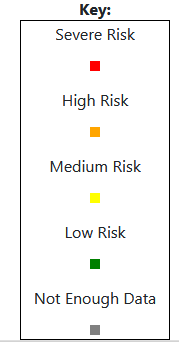
\includegraphics[scale=0.5]{Key.png}
    \caption{The key for the risk dependency graph.}
    \label{fig:key}
\end{center}
\end{figure}

\subsection{Project Activity Prediction}
For the project activity prediction, data from the GitHub API was used \cite{noauthor_github_nodate}. The focus was on number of commits per month and time-to-fix issues as these were identified as indicators of a project's activity and thus it's success \cite{sen_open_2012, chahal_fuzzy_2016}. The user has the option to specify whether they wish to investigate the issue, commit data or both. All of the data available was used instead of specifying a specific time range as all of the projects had different time ranges available to use. All of the commits/closed issues available were gathered using the GitHub API and this was processed to ensure there was data for each month up until the current date. In the case of commits, this was simply a count of commits per month and we added a 0 for each of the months with no data. For the issue data, the time-to-close in days was gathered for each issue and a monthly average was calculated, adding a 0 for each of the months that had no data. 

For the prediction, the date was used as an index and after calculating the \textit{d} parameter by differencing the data until the p-value of the augmented \textit{Dickey–Fuller test (ADF)} test was below 0.05, the \textit{Partial Autocorrelation Function (PACF)} and \textit{Autocorrelation function (ACF)} graphs were also examined it was not feasible to implement this system of parameter selection at a large scale. The \textit{Auto ARIMA} library was used to make the predictions as it offered a more useful manner of selecting parameters when predicting across many projects \cite{noauthor_pmdarima_nodate}. The final value predicted for the current month was returned for each of the GitHub libraries. If the data is constant or there is no data a -1 was returned as there is not enough data to make a prediction. 

\subsection{Vulnerability CVE Data Prediction}
For the vulnerability CVE data prediction vulnerability data from the NVD API was used \cite{noauthor_vulnerability_nodate}. The dependencies were then split into keywords to ensure that all of the relevant CVEs for that dependency were gathered. For each of the keywords, a request is made to the API and it is ensured that each of the returned CVEs is not in the already gathered list of CVEs. The monthly data, similar to the commits above, was gathered and the number of commits per month was counted and a 0 was filled in where there are none. 

The prediction method used was very similar to the project activity method. Some dependencies do not have many vulnerabilities per month or even per year. As there is not a lot of data for the vulnerability prediction section, it can be assumed if the values are constant or there is no data that there will be no vulnerabilities that month and return a 0. The \textit{Auto ARIMA} library was used in this case to make the predictions as above for feasibility it did not make sense to examine PACF and ACF graphs for each of the dependencies \cite{noauthor_pmdarima_nodate}. 


\subsection{Risk Calculations}
In order to calculate the risk, some configuration options were defined for a user to decide how many commits, days-to-close issues, and vulnerabilities per month are acceptable. These can be added to in the future if other risk metrics are needed. 

\[ projectActivityScore = ( x / numDaysToFixIssues ) * 10\]

\[ projectActivityScore = ( numCommits / x ) * 10\]

\[vulnerabilityScore = ( x / vulsCountPerMonth ) * 10\]

\begin{multline*}
  overallScore = ( projectActivityScore +\\ vulnerabilityScore) / 2 
\end{multline*}

\begin{table}
 \caption{Risk Score Levels}
\label{risklevels}
\begin{center}
\begin{tabular}{|c|c|c|}
\hline
    \textbf{Score} & \textbf{Risk Level} \\ \hline
    \textless  0 & Not Enough Data \\ \hline
    0 - 2.5 & Low Risk \\ \hline
    2.5-5 & Medium Risk \\ \hline
    5-7.5 & High Risk \\ \hline
    \textgreater 7.5  & Severe Risk \\ \hline
\end{tabular}
\end{center}
\end{table}

These are the calculations used for the risk scores. The idea was to calculate a score as defined above for project activity and a score for vulnerabilities and divide them by 2. There is the option to decide project activity based on issues fix time, commits per month or both. The user supplies the configuration options of \textit{numDaysToFixIssues}, \textit{numCommits}, and \textit{vulCountsPerMonth}. They set the acceptable levels of risk for their project. The idea is that they are then assigned a risk score: where not enough data is any number less than 0, 0-2.5 is low risk, 2.5-5 is medium risk, 5-7.5 is high risk and anything above 7.5 is a severe risk. These can be seen in table \ref{risklevels}. The overall score is then displayed on the graph - colour-coded using the key from Figure \ref{fig:key}. The appropriate levels of risk are left to the user to decide as some organisations/developers would have different ideas of what number is an acceptable number of commits/time to close issues/vulnerabilities per month. 

\begin{figure*}
    \centering
    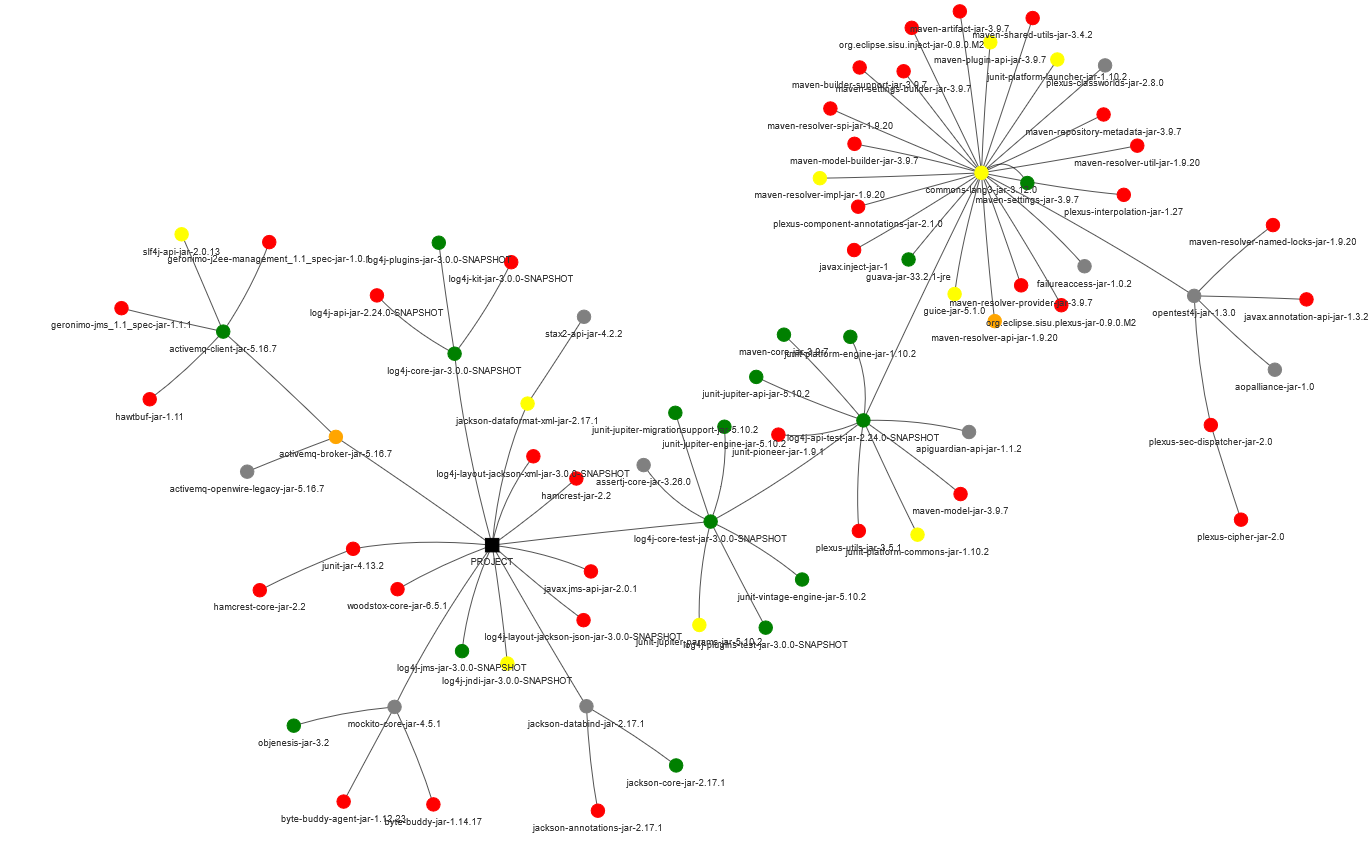
\includegraphics[scale=0.5]{dependency.png}
    \caption{Dependency tree results with risk levels colour coded.} 
    \label{fig:tree}
\end{figure*}
\section{Results}

In this section, the results obtained with this tool as well as some examples of the resulting graphs will be discussed. One particular Log4j sample project \cite{noauthor_logging-log4j-sampleslog4j-server_nodate} that was tested will be the focus, although a number of different types of projects were tested in addition to this to establish a baseline for the functionality of the graphing. By testing different types of projects, different dependencies were tested for risk. The baseline for the graphing was to establish feasibility for this project. First, the risk dependency visual that was created is examined and then two examples of the predictions made - one for project activity and one for vulnerability predictions. Prediction graphs for different dependencies are explored to give an idea of how accurate the predictions can be for both types of prediction. 

Figure \ref{fig:tree} shows a final dependency tree with colour-coded risk evaluations of each of the dependencies. This figure was based on a user configuration of two vulnerabilities being acceptable and 70 being the minimum number of commits per month as acceptable. It is clear there are a number of lower-level dependencies which are risky which the user may not be expecting. The graph is interactive so each specific dependency can be zoomed in on. If the graphs are larger or more dense the user can pick out specific risky nodes and choose to investigate their dependencies further or even compare different dependencies. 

\begin{figure}
    \centering
    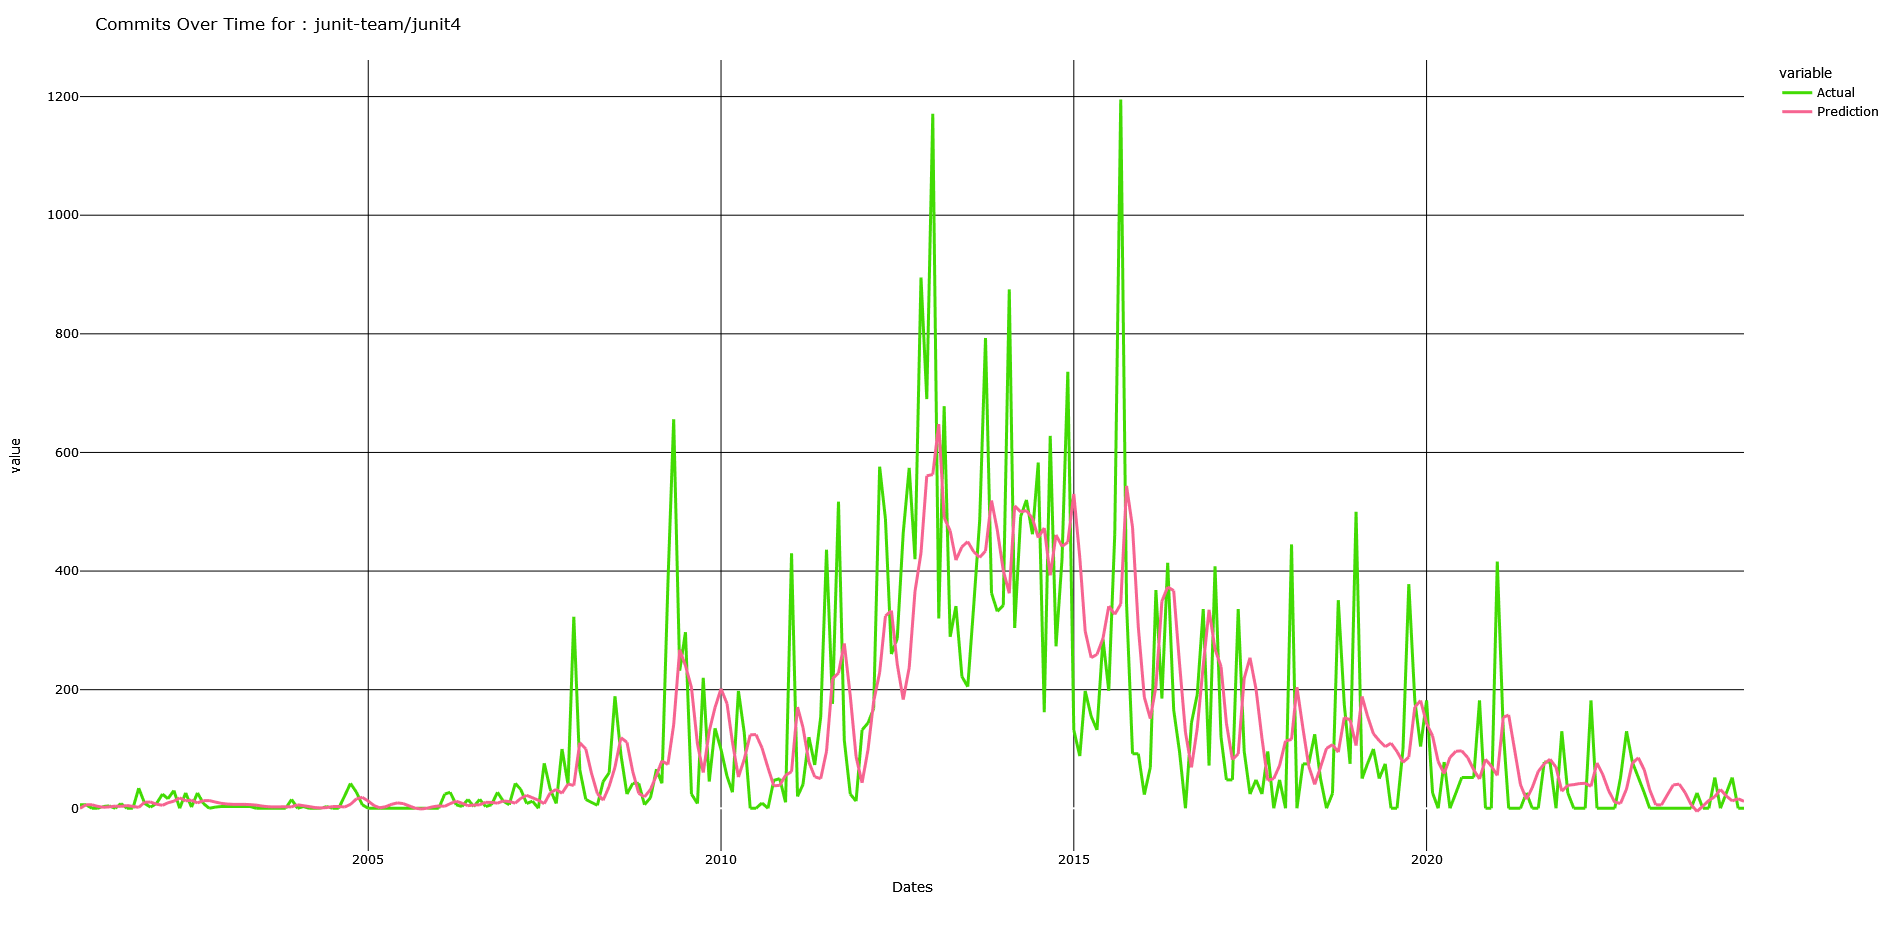
\includegraphics[width=1\linewidth]{JUnit4commits.png}
    \caption{Commits Per Month for JUnit4: Actual vs Predicted.} 
    \label{fig:commits}
\end{figure}

Figure \ref{fig:commits} shows the commits per month prediction vs actual values for the JUnit4 package. It is clear from this graph that the project activity in terms of commits was at its highest from around 2012 to 2017. 

\begin{figure}
    \centering
    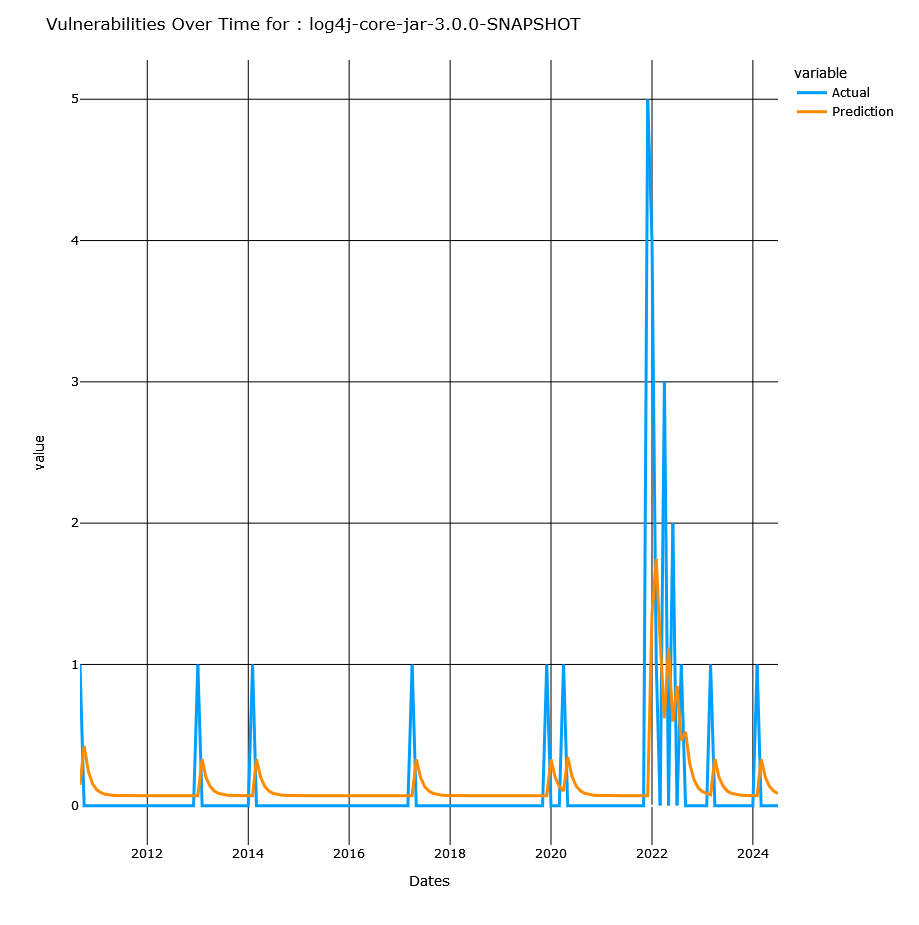
\includegraphics[width=1\linewidth]{Log4jVuls.png}
    \caption{Vulnerabilities Per Month for Log4j: Actual vs Predicted.} 
    \label{fig:vulns}
\end{figure}

Figure \ref{fig:vulns} shows the vulnerabilities for Log4j over time and it is clear to see where the Log4j vulnerabilities were released in 2021 and these are predicted reasonably well in the subsequent months. 

The tool displays graphs for every one of the predicted sets of data made. If there is not enough data for the prediction to be made then there is no corresponding graph. The idea is that the user can then investigate how accurate the predictions are for each of the graphs. For graphs with less data over time, the predictions did not perform well and occasionally there were constant lines being returned rather than actual predictions which could not be returned as a value for the risk dependency graph. An example of this can be seen in Figure \ref{fig:const}. The predicted values for the vulnerability data for the Jackson databind dependency. The predicted values are a constant value of just below 1 which is not accurate given the actual values. 

\begin{figure}
    \centering
    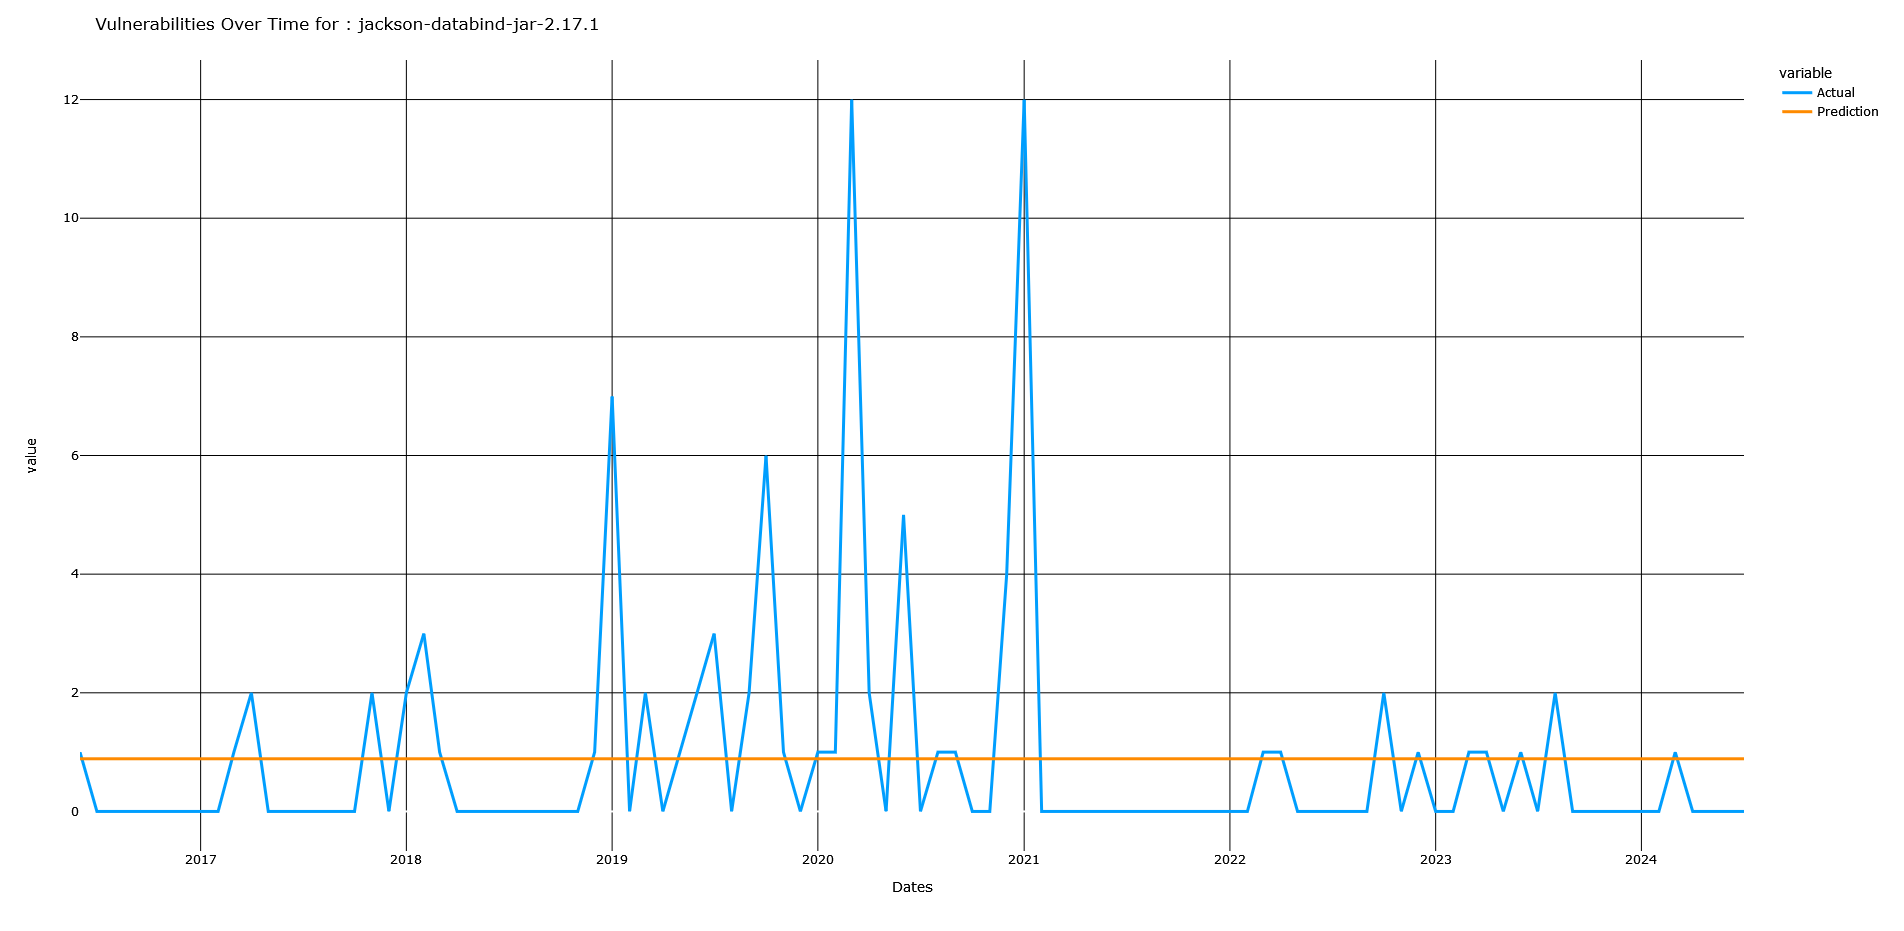
\includegraphics[width=1\linewidth]{Const.png}
    \caption{Vulnerabilities Per Month for Jackson databind: Actual vs Predicted.} 
    \label{fig:const}
\end{figure}

\section{Discussion}
In this section, we will discuss our progress in answering the research questions outlined in the Introduction. 

The first research question was whether features could be combined from the popular risk prediction methods to provide developers with a more complete risk measurement. The combination of risk prediction methods aided in identifying high-risk modules in dependency trees. Many of the dependencies investigated did not have any vulnerabilities reported in the NVD which is a desirable trait in any dependency. They were also, however, some dependencies no longer under development which means if a vulnerability were discovered in a non-surviving project it was unlikely to be fixed. This may not be an issue for large organisations that incorporate open-source software and configure it to meet their needs but smaller organisations lacking the resources to rework open-source software, may prefer to incorporate software that is still actively under development.

The second research question was whether the creation of a visual predicted risk dependency graph would be feasible. Some smaller projects were used to test the described tool but due to the zooming functionality of the graph, it would be feasible to create a similar graph for a larger dependency graph such as one used in industry. The developer could explore any nodes marked red and zoom in to discover which dependencies they are. The issue that the project may run into in this case is that the linking from dependencies to URLs for GitHub projects that used was gathered manually so it may become an issue with larger dependency lists as the list of links would be required to be more extensive. This could be avoided if there was an automatic system of gathering links for GitHub projects as we explore further in the future work section. 

\section{Performance Evaluation}
To evaluate the algorithm, a number of Maven projects were selected with varying dependencies. A sample Log4j maven project was used. 

The project activity predictions generally performed significantly better than the vulnerability CVE data - due to a lack of data in the NVD databases (which can in some cases mean no vulnerabilities - a positive). Numerous dependencies were also grouped in the same projects on GitHub which meant that there was only the need to calculate their associated project risk once. One issue encountered in testing was that there was no way of automatically using an API to find the GitHub project repositories of the dependencies - this meant the project URLs on GitHub had to be manually gathered by searching through each of the dependency trees which does not bode well for scaling the project up for larger Maven projects. 

For the evaluation of the models in this project, two commonly used metrics, mean absolute error (MAE), and root mean squared error (RMSE) were applied. 

\[ MAE = (1/n) \sum{i=n} |actual - forecast| \]

\[ RMSE = \sqrt( (\sum (forecast - predicted) ^ 2) / sample size )  \]

These are the most commonly used evaluation metrics when evaluating Time Series predictions such as ARIMA. MAE is simply the mean of absolute errors where the absolute error is the difference between actual and predicted values. RMSE measures the standard deviation of the residuals and their dispersion. It is the commonly used metric to evaluate the difference between actual and forecasted values. This measurement can be heavily influenced by any outlier predictions \cite{f_abdulhafidh_dael_performance_2022}. We investigated the use of mean absolute percentage error (MAPE) but we found this was not suitable as some of the actual values were 0. It is a measure of the average of the percentage error and will produce extreme values if the actual value is quite small and in the case of the actual value being a 0 the result is always Infinite. Through the use of these evaluation metrics, an understanding can be gained of the performance of our time series models. 

\begin{table}
 \caption{Evaluation of Predictions}
\label{evaluations}
\begin{center}
\begin{tabular}{|c|c|c|c|}
\hline
    \textbf{Prediction} & \textbf{MAE} & \textbf{RMSE} \\ \hline
    Commits per month & 123.18 & 213.96 \\ \hline
    Vulnerabilities per month & 0.15 & 0.48 \\ \hline
\end{tabular}
\end{center}
\end{table}

The evaluation we obtained for the two figures above fig \ref{fig:commits} and fig \ref{fig:vulns} can be seen in Table \ref{evaluations}. The figures show that the evaluation metrics of the vulnerability prediction are better than those of the commits per month prediction. This may be due to the high number of commits over time vs the low number of vulnerabilities. Considering the Log4j vulnerability caused a large spike in vulnerabilities being released for this package, the vulnerability prediction performs quite well and seems to take these spikes into account when predicting the next values. 

\subsection{Threats to Validity}
In this section, we identify possible threats to the validity of the results we obtained and how they were addressed. 

\subsubsection{Dataset}
The dataset used was quite limited. Several small Maven projects were used to test the initial design. This was to ensure that the analysis was tractable and test the code rapidly and efficiently generate the graphs. The analysis takes significant time to run for larger projects - although the data gathering takes up the largest proportion of time. To combat the lack of available datasets and the manual work gathering GitHub URLs a sample Log4j Maven project was analysed as this had known vulnerabilities and thus had a spike in fixes and project activity. Another dataset issue was that there was a scarcity of vulnerability data per month in the same way that there was for the project activity. As discussed above, the resulting vulnerability predictions were not always the most accurate. 

\subsubsection{AutoARIMA}
The use of manual ARIMA prediction was investigated but this meant PACF and ACF plots for each of the predictions would need to be investigated which was unfeasible for some of the larger dependency trees. It was found to be reasonably simple to calculate the differencing parameter calculated but very difficult to calculate the others. The use of the AutoARIMA predictions means the predictions are not as accurate as they could be for every dataset but as this project requires significant API usage and data processing for each of the dependencies (which can be a large number) it was preferable to implement an automatic system rather than manually analysing each dataset. The prediction made assumes that there is no seasonality in the datasets as this was reported in the literature to be of little significance \cite{roumani_time_2015}. 

\section{Conclusions \& Further Work}
The growing reliance on open-source software \cite{noauthor_cisa_2023} has introduced several challenges regarding the security and integrity of software supply chains. Tools to explore the risk in software supply chains like the one we proposed, designed and implemented as described in this paper we have demonstrated to be useful in identifying high risk open-source dependencies. As the reliance on open-source software grows, so does the need for tools such as ours. We set out to answer two research questions and our investigation concluded that the combination of the two measures of risk, both project activity and vulnerabilities over time gives a valuable overview of the risk in using a project. We have depicted risk visually in an interactive dependency graph. 

For the purpose of this paper, we focused on examining Maven dependency trees which are primarily used for Java projects. Further work to examine other package manager dependency trees such as \textit{PyPI} for Python, \textit{NPM} for JavaScript, and \textit{Conan} for C is clearly warranted. This may give a different perspective as different languages may be more prone to vulnerabilities or have projects which are less likely to survive. Java is known for having many third-party dependencies with vulnerabilities but it is also well known that C is more prone to vulnerabilities in source code so it may be useful to explore this question across multiple languages. 

Another avenue of future work would be to create an automatic method of gathering GitHub URLs for each of the dependencies as the lack of such a system meant we were limited in the amount of testing that we could carry out. An automatic tool like this would be useful in other contexts such as finding other details about project activity or the latest versions. This would make the project activity prediction for this project a lot simpler and would increase its scalability when analysing larger projects. 

In general, the performance of our tool was reasonably accurate in terms of the prediction of both vulnerabilities per month and project activity. We compromised on the accuracy of our predictions in order to ensure that we could obtain reasonably accurate predictions for many dependencies without having to analyse each individually. As a result, the tool can scale up when making predictions for any type of project. We kept the tool configurable so users could set the level of risk that they deem appropriate. There remains scope to investigate other project activity metrics such as the number of remaining contributors which was an important factor in the literature for the survival of an open-source project \cite{l_bao_large_2021}. The vulnerability aspect of the project can also be configured so that users can choose their own risk levels to suit their context. The aim of this project was to highlight to users high-risk modules in their Maven dependency trees so that they can opt for more secure modules when comparing open-source software. We have demonstrated that a tool like ours could aid developers in choosing modules which are less risky and in discovering high-risk unknown dependencies. While our project is currently limited in its scalability due to the lack of an automatic way to associate GitHub repositories with Maven dependencies, we have shown our approach provides a solid foundation for future research in the area of securing the software supply chain. 

\bibliography{references}

\appendices

\section{Configuration Options JSON}
This listing shows an example of how the configuration options can be set. 

\begin{lstlisting}[caption=Configuration Options]
{
  "num_vuls": "2",
  "num_days_to_fix": "46",
  "num_commits": "70",
  "issues_or_commits": "commits",
  "token": "",
  "nvd_key": ""
}
\end{lstlisting}

\section{Dependencies Comparison}
This figure \ref{fig:comp} shows the tool being used to compare two similar dependencies and it is clear to see that Mockito is the safer option when compared to JUnit4 according to the parameters set. 

\begin{figure}[H]
    \centering
    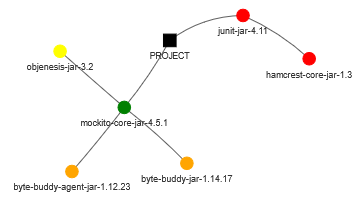
\includegraphics[width=1\linewidth]{Comparison.png}
    \caption{Comparison of Unit Testing Dependencies: Mockito vs JUnit4.} 
    \label{fig:comp}
\end{figure}

\newpage

\section{Dependency Tree Example}
The following listing shows a Maven dependency example used to test this project. 

\begin{lstlisting}[caption=Example Maven dependencies]
[INFO] Scanning for projects...
[INFO] 
[INFO] --------------------------< org.youtube:form >--------------------------
[INFO] Building form 1.0-SNAPSHOT
[INFO]   from pom.xml
[INFO] --------------------------------[ jar ]---------------------------------
[INFO] 
[INFO] --- dependency:3.6.0:tree (default-cli) @ form ---
[INFO] org.youtube:form:jar:1.0-SNAPSHOT
[INFO] +- org.openjfx:javafx-controls:jar:16:compile
[INFO] |  +- org.openjfx:javafx-controls:jar:win:16:compile
[INFO] |  \- org.openjfx:javafx-graphics:jar:16:compile
[INFO] |     +- org.openjfx:javafx-graphics:jar:win:16:compile
[INFO] |     \- org.openjfx:javafx-base:jar:16:compile
[INFO] |        \- org.openjfx:javafx-base:jar:win:16:compile
[INFO] +- org.openjfx:javafx-fxml:jar:16:compile
[INFO] |  \- org.openjfx:javafx-fxml:jar:win:16:compile
[INFO] +- org.eclipse.persistence:eclipselink:jar:2.7.7:compile
[INFO] |  +- org.eclipse.persistence:jakarta.persistence:jar:2.2.3:compile
[INFO] |  \- org.eclipse.persistence:commonj.sdo:jar:2.1.1:compile
[INFO] +- org.eclipse.persistence:javax.persistence:jar:2.0.0:compile
[INFO] \- org.postgresql:postgresql:jar:9.3-1102-jdbc41:compile
[INFO] ------------------------------------------------------------------------
[INFO] BUILD SUCCESS
[INFO] ------------------------------------------------------------------------
[INFO] Total time:  1.360 s
[INFO] Finished at: 2024-05-19T20:49:23+01:00
[INFO] ------------------------------------------------------------------------


\end{lstlisting}


\ifCLASSOPTIONcaptionsoff
  \newpage
\fi

\end{document}